\secnumbersection{PROPUESTA DE SOLUCIÓN}\label{ch:propuesta_solucion}

El presente capítulo detalla el diseño, la estructura de la metodología y la implementación del sistema propuesto para la sonificación de datos de \textit{4D Flow MRI}. Para garantizar la escalabilidad y coherencia física de los resultados, el desarrollo de la solución no se abordó como un proceso único, sino que se fue dividido en 3 etapas, las cuales dictan la organización de este capítulo 

\begin{enumerate}
    \item \textbf{Exploración espacial y síntesis acústica:} Esta etapa está enfocada en el preprocesamiento de los datos anatómicos y su traducción acústica. Se detallan la integración del \textit{centerline}, su interpolación espacial, el cálculo iterativo de los planos de corte ortogonales y la formulación trigonométrica para extraer las proyecciones de velocidades. Además, se describe el motor de la síntesis digital de señales encargado de mapear la cinemática del fluido a parámetros sonoros. Todo el procesamiento se consolida dentro de una interfaz gráfica interactiva, la cual permite la inspección y exploración de los diferentes planos y sus flujos. 
    
    \item \textbf{Procesamiento masivo y extracción de características:} Esta segunda etapa se centra en la automatización del flujo de trabajo y la consolidación de la información. Se detalla la implementación de rutinas de procesamiento por lotes (\textit{batch processing}) para extraer y almacenar de forma masiva las proyecciones de velocidad de los diferentes casos de estudio que se ingresan al sistema. La etapa concluye con la construcción de un conjunto de datos estructurado (\textit{dataset}) mediante la extracción automatizada de descriptores correspondientes tanto a la cinemática del fluido como a la síntesis acústica.

    \item \textbf{Esquema de análisis cuantitativo y exploración interactiva:} Constituye la etapa final, destinada a corroborar la eficacia de la herramienta de sonificación. Por un lado, se establece un diseño de agrupamiento estadístico sobre el conjunto de características estructurado para analizar objetivamente la correlación de las variables. Por otro lado, se detalla la arquitectura de un tablero interactivo (\textit{dashboard}) para la exploración perceptiva, permitiendo la comparación simultánea de escenarios hemodinámicos con el fin de comprobar empíricamente si las alteraciones del flujo se traducen en firmas acústicas predecibles y distinguibles.
\end{enumerate}

\subsection{Exploración espacial y síntesis acústica}

La primera etapa del sistema se centra en el acondicionamiento de los datos y la configuración del motor de extracción espacial. El objetivo de esta fase es aislar secciones transversales del vaso sanguíneo para poder evaluar el comportamiento hemodinámico de forma iterativa y secuencial a lo largo de toda la estructura anatómica.


\subsubsection{Interpolacíon del \textit{centerline} y cálculo de planos ortogonales}

El flujo de procesamiento se inicia con la ingesta de los datos espaciales derivados de la resonancia magnética (\textit{4D Flow MRI}). Entre los datos de entrada, el sistema recibe la segmentación anatómica del vaso y una matriz de coordenadas precalculada correspondiente al \textit{centerline}.

Dado que las coordenadas originales del \textit{centerline} se encuentran expresadas en el espacio discreto de la matriz de imagen, el primer paso consiste en transformar estos datos al espacio físico real. Para ello, cada componente cartesiana de la curva se multiplica por la resolución espacial del escáner, definida por el tamaño del vóxel en sus dimensiones $X$, $Y$ y $Z$. Esta operación de escalado permite transicionar del dominio de los píxeles a una métrica en milímetros.

Una vez proyectada en el espacio físico, la curva original puede presentar un muestreo irregular para realizar un análisis continuo. Para estandarizar la topología del vaso, el sistema aplica una interpolación paramétrica mediante trazadores cúbicos (\textit{cubic splines}). Este procedimiento genera una nueva curva espacial suave, de la cual se extrae una resolución espacial de 90 puntos de estudio equidistantes. Cada coordenada interpolada $P_i = (x_i, y_i, z_i)$, con $i \in \{1, 2, \dots, 90\}$, representa el centro geométrico exacto de la región de interés para una iteración de análisis.

Para extraer de manera fidedigna la información hemodinámica en un punto de estudio $P_i$, es estrictamente necesario seccionar los volúmenes de velocidad utilizando un plano que sea perpendicular a la dirección longitudinal del vaso en ese instante específico. La orientación geométrica de este plano oblicuo queda definida por un vector normal $\vec{N}_i$. 
 
La definición de este plano ortogonal se vincula directamente con el principio físico del \textbf{ángulo de insonación} ($\theta$) descrito en el marco teórico. En ultrasonido Doppler, este ángulo —formado entre el haz acústico y la dirección del flujo sanguíneo— dicta la exactitud de la velocidad medida a través del factor de corrección $\cos(\theta)$. Al diseñar el plano de corte de manera estrictamente perpendicular a la línea central del vaso, el sistema garantiza que el vector normal $\vec{N}_i$ se mantenga paralelo a la dirección principal del flujo sanguíneo. Esta decisión de diseño equivale a establecer un escenario de exploración ideal con un ángulo de insonación computacional tendiente a $0^\circ$ ($\cos(0^\circ) = 1$), lo que maximiza los valores de \textit{Doppler shift} medidos.

Computacionalmente, este vector director se estima evaluando la derivada posicional mediante una aproximación de diferencias finitas con los puntos adyacentes de la curva interpolada:

$$\vec{N}_i = P_{i+1} - P_{i-1}$$

Donde $P_{i+1}$ y $P_{i-1}$ corresponden al punto posterior y anterior en la secuencia espacial del vaso, respectivamente. En los extremos anatómicos (el primer y el último punto), el cálculo se ajusta utilizando el punto actual y su único vecino disponible. La correcta definición del origen del plano $P_i$ y su vector normal $\vec{N}_i$ proporciona los parámetros exactos requeridos para aislar y proyectar las velocidades tridimensionales del fluido, proceso que constituye el núcleo del motor de extracción.


\subsubsection{Extracción geométrica y proyección de velocidades}

Una vez establecidos el origen del plano $P_i$ y su vector normal $\vec{N}_i$ en una iteración dada, el sistema normaliza este vector para obtener un vector director unitario $\hat{n}_i = \frac{\vec{N}_i}{||\vec{N}_i||}$. Este vector unitario es fundamental para garantizar que las transformaciones geométricas subsecuentes preserven las magnitudes físicas originales del fluido.

Con los parámetros espaciales definidos, el sistema ejecuta la sección de las matrices volumétricas correspondientes a las tres componentes espaciales de la velocidad capturadas por el resonador ($V_x$, $V_y$, $V_z$, muchas veces representadas por $V_RL$, $V_AP$ y $V_FH$). Esta se implementa mediante la extracción de un corte oblicuo (\textit{oblique slice}) a través de los volúmenes tridimensionales. La matriz bidimensional resultante contiene, en cada uno de sus píxeles, un vector de velocidad tridimensional $\vec{V} = (v_x, v_y, v_z)$ que describe el movimiento del fluido en esa región transversal específica.

Sin embargo, el realizar un corte oblicuo sobre la segmentación anatómica, la representación resultante no siempre es una región única. Con frecuencia presenta múltiples regiones aisladas o \textit{islas}. Estas discrepancias topologícas pueden ser producto de ruido inherente en la imagen, ramificaciones vasculares secundarias o vasos sanguíneos adyacentes que cruzan el mismo plano de corte.

Para aislar de manera efectiva la estructura de interés, el sistema implementa un algoritmo de etiquetado de componentes conexos (\textit{connected-component labeling}). Esta operación analiza la conectividad espacial de los píxeles y asigna una etiqueta discreta a cada agrupación independiente. A continuación, el algoritmo evalúa las propiedades geométricas de cada componente detectado —específicamente su área superficial y la distancia topológica hacia la coordenada interpolada de la línea central $P_i$—. Mediante este análisis, el sistema selecciona y extrae exclusivamente la componente conexa principal, descartando automáticamente cualquier artefacto o estructura vascular paralela.

Muchas veces los vóxeles ubicados en la periferia anatómica del vaso son altamente propensos a sufrir efectos de volumen parcial (\textit{Partial Volume Effect, PVE}), presentando una baja relación señal-ruido. Para evitar que estas mediciones introduzcan artefactos, a la región aislada se le aplica una operación de erosión que descarta las capas de píxeles más externas.

Esta nueva máscara depurada se utiliza entonces como un filtro lógico sobre las matrices de velocidad cortadas, enmascarando con valor nulo todos los píxeles fuera de la región segura. Como resultado, se obtiene una matriz tridimensional $\vec{V} = (v_x, v_y, v_z)$ que contiene vectores cinemáticos de alta fidelidad.

Sin embargo, el ultrasonido Doppler no evalúa campos vectoriales tridimensionales, sino que registra únicamente la componente de la velocidad paralela al eje de insonación. Para emular computacionalmente esta restricción física y transformar el dato volumétrico en una señal unidimensional, el sistema ejecuta un proceso de proyección ortogonal en dos etapas: aislamiento escalar y recuperación de la direccionalidad.

En primera instancia, el algoritmo calcula la proyección vectorial de la velocidad tridimensional sobre el vector normal unitario del plano. Matemáticamente, esto se formula extrayendo el vector proyectado $\vec{V}_{proj}$ y calculando su magnitud absoluta o norma euclidiana:

$$||\vec{V}_{proj}|| = ||(\vec{V} \cdot \hat{n}_i) \hat{n}_i|| = \sqrt{V_{px}^2 + V_{py}^2 + V_{pz}^2}$$


Esta magnitud $||\vec{V}_{proj}||$ representa la velocidad neta del flujo a lo largo del eje, pero carece de sentido direccional al ser un valor estrictamente positivo. Para determinar si el flujo se acerca o se aleja del plano, el sistema implementa una evaluación trigonométrica. Se calcula el cociente entre el producto escalar del vector proyectado con la normal y su magnitud absoluta, limitando el resultado al rango $[-1, 1]$ para evitar inestabilidades numéricas. Al evaluar el arcoseno de este cociente, el algoritmo extrae un factor de signo correspondiente a las orientaciones ortogonales extremas ($+90^\circ$ o $-90^\circ$).

Al normalizar este ángulo y multiplicarlo por la magnitud absoluta previa, el sistema genera la velocidad proyectada final ($V_p$). Mediante esta secuencia algorítmica y trigonométrica, se logra colapsar la complejidad del \textit{4D Flow MRI} en un perfil bidimensional, direccional y libre de ruido perimetral, estableciendo la entrada directa para el motor de sonificación.

\subsubsection{Construcción espectral y síntesis acústica}

El núcleo del sistema radica en la traducción de las velocidades proyectadas hacia el dominio auditivo y visual. El sistema emula la física detrás del ultrasonido Doppler generando un espectrograma y luego se realiza la síntesis. 

En la práctica, el espectrograma Doppler representa la distribución temporal de las velocidades del flujo. Para emular correctamente esta firma, el sistema construye una matriz espectral virtual analizando la matriz bidimensional de velocidades proyectadas a lo largo de las distintas fases del ciclo cardíaco.

El proceso se inicia definiendo dinámicamente los límites de la escala de velocidad, calculando los percentiles extremos (0.5 y 99.5) de todas las mediciones transversales para descartar valores atípicos y asegurar una representación robusta. Posteriormente, para cada fase temporal temporal, se agrupan las velocidades en un histograma continuo de 128 niveles (\textit{bins}). Este conteo captura la densidad de la sangre (cantidad de vóxeles) moviéndose a cada rango de velocidad.

Para asegurar una transición fluida en la representación visual, el algoritmo interpola las fases temporales discretas del \textit{4D Flow MRI} hacia el dominio de muestreo de audio de alta resolución mediante trazadores polinómicos (\textit{splines}). Finalmente, a la matriz resultante se le aplica una compresión no lineal mediante un factor Gamma ($\gamma = 0.65$):

$$M_{ij}' = M_{ij}^\gamma$$

Esta corrección Gamma es fundamental, ya que expande visualmente las intensidades bajas del histograma, permitiendo al observador distinguir componentes de flujo sutiles que de otro modo quedarían enmascarados por las velocidades dominantes.

Mientras que la matriz espectral gestiona la representación visual, la generación del audio se fundamenta en el principio físico del \textit{Pulsed Wave Doppler, PW}. Esto se debe a que se emula el comportamiento de una compuerta de muestra (\textit{sample volume} o \textit{gate}) al evaluar de forma aislada las velocidades contenidas en un plano transversal específico ($P_i$).

Para la síntesis acústica de esta sección espacial, el algoritmo calcula el \textit{Doppler shift} ($\Delta f$) de cada vóxel basándose en la ecuación del ultrasonido Doppler (ver Sección \ref{subsection:doppler_ultrasound}). En esta implementación, la variable $v$ corresponde a la velocidad proyectada. Asimismo, los parámetros operativos del transductor virtual se fijan en $f_0 = 1.25$ MHz para la frecuencia de emisión emulada y $c = 154,000$ cm/s para la velocidad de propagación del sonido en el tejido blando.

Una vez definido el \textit{Doppler shift} instantáneo, el sistema calcula la fase acústica acumulada integrando numéricamente la variación de la frecuencia a lo largo del tiempo del latido cardíaco (ver Sección \ref{subsection:integracion_fase}).

Finalmente, la onda acústica base de cada vóxel se genera evaluando la función coseno sobre su respectiva fase acumulada ($\cos(\Phi(t))$). Esta operación transforma la cinemática aislada de la resonancia en oscilaciones mecánicas virtuales, dejándolas listas para la consolidación del sonido final. Una vez calculadas las ondas cosenoidales individuales para cada vóxel de la región transversal, el sistema consolida el audio global del plano mediante la técnica de síntesis aditiva.

Previo a la sumatoria, el sistema implementa una espacialización dinámica basada en la dirección del flujo. Se utiliza una función tangente hiperbólica ($\tanh$) sobre las velocidades proyectadas para calcular coeficientes de ponderación estéreo. Este enfoque permite enrutar suavemente los flujos anterógrados (velocidades positivas) hacia el canal derecho y los flujos retrógrados (velocidades negativas) hacia el canal izquierdo, emulando la separación direccional presente en el \textit{hardware} de un ecógrafo real:

$$ W_{der} = 0.5 \cdot \left(1 + \tanh(v(t))\right) $$
$$ W_{izq} = 1 - W_{der} $$

La consolidación del sonido se logra multiplicando cada onda acústica individual por su respectivo peso espacial y aplicando la sumatoria a todas las componentes. Esta operación materializa la síntesis aditiva:

$$ S_{der}(t) = \sum_{i=1}^{N} \cos(\Phi_i(t)) \cdot W_{der, i} $$
$$ S_{izq}(t) = \sum_{i=1}^{N} \cos(\Phi_i(t)) \cdot W_{izq, i} $$

Previo a la etapa final de filtrado, la señal acústica debe ser moldeada para reflejar la dinámica del ciclo cardíaco. Para ello, el sistema calcula una envolvente temporal de amplitud basada en la sumatoria del flujo absoluto que atraviesa el plano transversal en cada fase. Esta curva es sometida a un suavizado gaussiano para evitar transiciones bruscas que generen clics digitales. Al multiplicar la señal de audio estéreo por esta envolvente, se garantiza que la presión sonora resultante sea directamente proporcional a la energía cinética del fluido, produciendo incrementos de volumen en sístole y atenuaciones en diástole.

Para maximizar el realismo acústico, la señal es sometida a un procesamiento final de filtrado y modulación. En primer lugar, se emula el ``golpe de pared'' (\textit{Wall Thump}), un artefacto sonoro de baja frecuencia producido por la distensión mecánica de la pared vascular durante la sístole. El algoritmo calcula la aceleración global del flujo y la utiliza para modular la amplitud de una señal estocástica grave, integrando este impacto característico al audio principal.

Finalmente, aplicando los principios de la síntesis sustractiva, las señales estéreo transitan por una etapa de filtrado digital discreto. Se implementan filtros tipo Butterworth de fase cero (\textit{filtfilt}) para esculpir la señal acústica sin introducir distorsiones de retardo temporal:

\begin{itemize}
    \item \textbf{Filtro de pared (\textit{High Pass}):} Se aplica una frecuencia de corte de 150 Hz para suprimir componentes de muy baja frecuencia.     

    \item \textbf{Filtro de paso bajo (\textit{Low Pass}):} Con una frecuencia de corte fijada en 1200 Hz, este filtro actúa como un limitador de banda para suavizar la respuesta acústica y eliminar artefactos de aliasing digital. 
\end{itemize}

El resultado de esta cadena de procesamiento algorítmico es una señal estéreo bidireccional y depurada, que recrea con alta fidelidad tanto la cinemática de los datos del \textit{4D Flow MRI} como las características sonoras del ultrasonido Doppler .

\subsubsection{Consolidación visual y exploración}

La matemática y síntesis de sonido descrita anteriormente se encapsula dentro de una interfaz gráfica de usuario, diseñada para la exploración de la estructura vascular. Este panel, ilustrado en la Figura \ref{fig:explorador_gui}, se divide en 3 visores principales sincronizados dinámicamente:

\begin{itemize}
    \item \textbf{Visor anatómico 3D:} Esta parte de la interfaz renderiza una isosuperficie (\textit{isosurface}) semi-transparente de la matriz de segmentación del vaso sanguíneo, superponiendo el \textit{centerline} interpolado. Un marcador espacial indica en tiempo real la coordenada exacta $P_i$ que está siendo procesada y su correspondiente corte oblicuo, proporcionando contexto topológico al usuario mediante un control deslizante.

    \item \textbf{Panel espectral:} Genera el espectrograma Doppler a partir de la matriz de velocidades proyectadas.
    
    \item \textbf{Panel acústico:} Grafica la forma de la onda (\textit{waveform}) de la señal de audio sintetizada.
\end{itemize}

\begin{figure}[H]
    \centering
    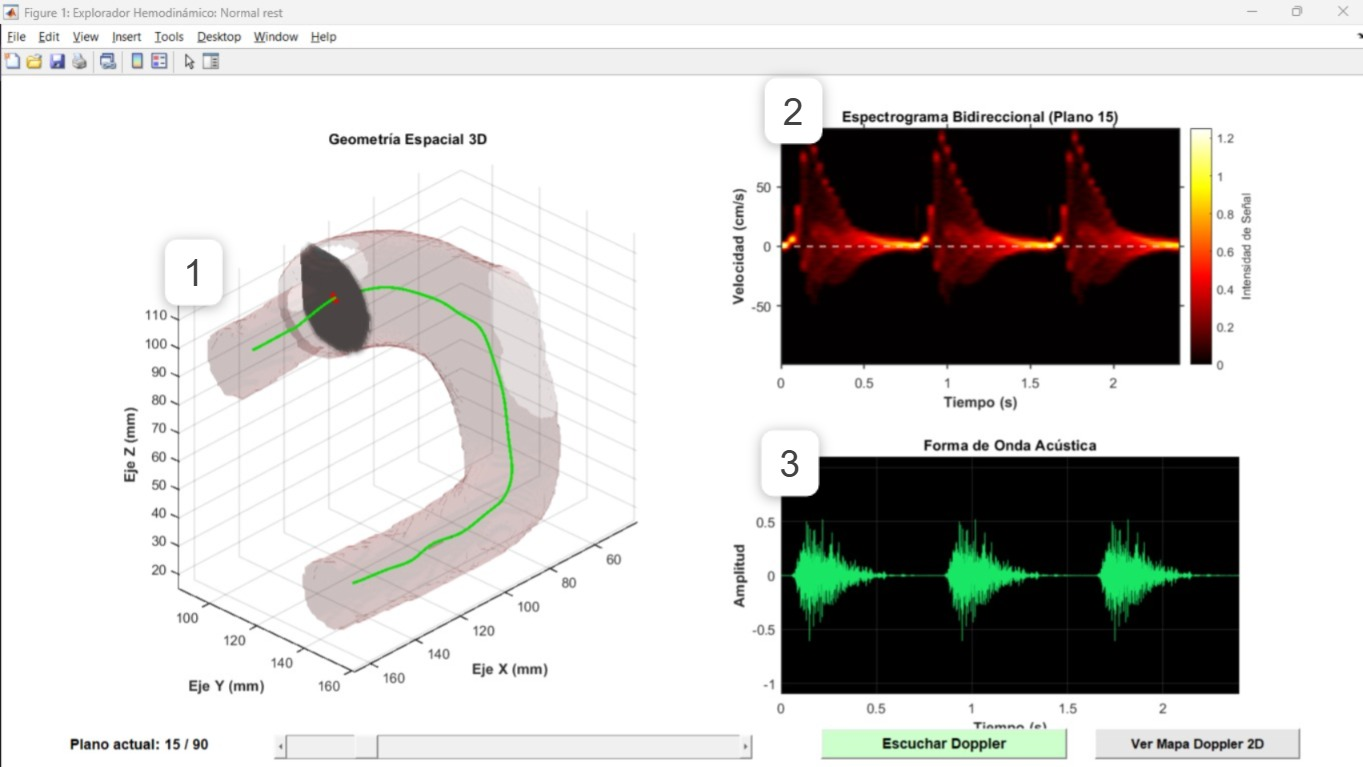
\includegraphics[width=0.9\textwidth]{figures/propuesta/explorador.jpeg}
    \caption{Interfaz del Explorador Hemodinámico: Dado un punto en el \textit{centerline} se renderiza el plano oblicuo de corte junto con la visualización anatómica (1), el panel espectral (2) y el panel acústico (3). Fuente: Elaboración propia.}
    \label{fig:explorador_gui}
\end{figure}

Adicionalmente, el sistema integra un módulo de visualización bidimensional que emula la modalidad de \textit{Color Doppler} cuyo resultado se presenta en la Figura \ref{fig:doppler_2d_gui}. A diferencia del espectrograma, que sintetiza el comportamiento dinámico del flujo en el tiempo, este módulo genera representaciones transversales para cada fase del ciclo cardíaco.

Mediante el uso de la máscara geométrica, el algoritmo proyecta las velocidades locales sobre un mapa de calor dinámico que codifica la información hemodinámica mediante una escala cromática dicotómica:
\begin{itemize}
\item \textbf{Tonalidades cálidas:} Representan el flujo anterógrado (velocidades positivas).
\item \textbf{Tonalidades frías:} Representan el flujo retrógrado (velocidades negativas).
\end{itemize}

En esta representación, la saturación del color escala proporcionalmente con la magnitud de la velocidad, permitiendo la identificación visual de gradientes hemodinámicos en la sección transversal del vaso.


\begin{figure}[H]
    \centering
    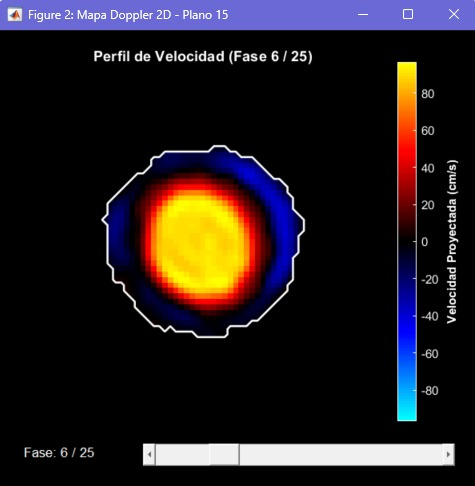
\includegraphics[width=0.65\textwidth]{figures/propuesta/doppler_2d.jpeg}
    \caption{Módulo que emula el \textit{Color Doppler} (Plano 15, Fase 6/25). Las tonalidades cálidas representan flujo anterógrado y las frías flujo retrógrado. Fuente: Elaboración propia.}
    \label{fig:doppler_2d_gui}
\end{figure}

\subsection{Procesamiento masivo y extracción de características}

La segunda etapa del desarrollo consiste en transicionar de una herramienta de exploración visual interactiva a un motor de medición automatizado. Para evaluar el impacto de diferentes morfologías y condiciones de flujo, es necesario extraer descriptores matemáticos discretos a partir de las matrices extraídas en la primera fase. Esta etapa detalla la optimización del procesamiento por lotes y la parametrización de las señales cinemáticas y acústicas.

\subsubsection{Procesamiento secuencial y gestión de memoria}

Dada la alta dimensionalidad de los volúmenes de \textit{4D Flow MRI}, la extracción manual de parámetros para las diferentes secciones transversales de cada modelo anatómico resulta inviable. Por ello, se implementó un algoritmo orquestador encargado de invocar el motor de extracción espacial de forma secuencial y autónoma para las diferentes fuentes de datos.

Durante este procesamiento masivo, el principal cuello de botella computacional es la saturación de la memoria volátil (RAM) al operar simultáneamente con múltiples matrices de gran tamaño. Para garantizar la escalabilidad, el sistema fue diseñado bajo una arquitectura de canalización (\textit{pipeline}): el orquestador ejecuta el corte y la proyección plano a plano, y exporta inmediatamente las matrices bidimensionales resultantes al almacenamiento local en formato de arreglos binarios. Este diseño transforma el modelo tridimensional pesado en un repositorio de datos ligero y fragmentado, permitiendo el procesamiento ininterrumpido sin comprometer la estabilidad del sistema computacional.

\subsubsection{Parametrización cinemática y acústica (\textit{Feature Extraction})}

Con las señales espaciales exportadas, el sistema ejecuta un módulo de parametrización encargado de traducir los campos vectoriales y las ondas de sonido en métricas escalares concretas. Para garantizar una comparación coherente a lo largo de toda la estructura, el sistema implementa una sincronización temporal dinámica basada en el caudal volumétrico.

Computacionalmente, la integración espacial del campo de velocidades se ejecuta mediante una sumatoria discreta de las magnitudes absolutas de todos los vóxeles válidos para cada fase temporal $t$:

$$ Q(t) = \sum_{j=1}^{N} |v_j(t)| $$

Donde $N$ es el número total de vóxeles que conforman el lumen en el plano transversal analizado, y $v_j(t)$ es la velocidad proyectada de cada vóxel. La utilización del valor absoluto en esta formulación es una consideración fundamental: garantiza que la presencia de flujos retrógrados o vórtices locales sumen a la energía cinética total de la sección en lugar de cancelarse matemáticamente con el flujo anterógrado.

Una vez construido el vector de caudal $Q(t)$ para todo el ciclo cardíaco, el algoritmo identifica el instante donde se alcanza el máximo valor del ciclo ($t_{sistole} = \arg\max Q(t)$). La fase temporal que satisface esta condición es etiquetada como el pico sistólico, estableciendo el punto de medición estándar para la extracción de características estáticas.

La extracción de parámetros se divide en dos dominios complementarios:

\textbf{Métricas de la dinámica de fluidos:} Estos parámetros cuantifican la física del flujo a partir de la cinemática volumétrica del latido:
\begin{itemize}
    \item \textbf{Velocidad máxima ($V_{max}$) y media ($V_{mean}$):} La velocidad máxima se obtiene utilizando el percentil 99.5 de la distribución de velocidades del plano en el pico sistólico. La aplicación de este límite probabilístico, en lugar del valor máximo absoluto, es una contramedida algorítmica para mitigar el impacto de valores anómalos (\textit{outliers}) propios del ruido de la resonancia.
    
    \item \textbf{Varianza y asimetría espacial (\textit{Skewness}):} Describen estadísticamente la distribución de los gradientes de velocidad transversal. Valores elevados indican una alteración del perfil parabólico normal, caracterizando la pérdida de laminaridad, flujos caóticos o zonas de recirculación.
    
    \item \textbf{Índice de pulsatilidad (PI):} Parámetro hemodinámico clásico calculado a partir de la evolución temporal de todo el ciclo cardíaco, relacionando la amplitud de la velocidad (sístole menos diástole) con la velocidad media del ciclo.
\end{itemize}

\textbf{Métricas de la señal digital:} Aprovechando el motor de síntesis, las proyecciones espaciales se transforman en señales de audio. Para estandarizar el análisis, la señal es truncada a una ventana de observación correspondiente a exactamente un ciclo cardíaco. Sobre esta onda modulada se extraen los siguientes descriptores de audio digital:
\begin{itemize}
    \item \textbf{Análisis en el dominio del tiempo:} Se calcula la energía cuadrática media (\textit{RMS}) y la tasa de cruces por cero (\textit{Zero-Crossing Rate, ZCR}). Estas variables traducen la presión sonora aparente y la densidad de fluctuaciones de la señal acústica\cite{eronen2000musical}.
    
    \item \textbf{Análisis en el dominio de la frecuencia:} Mediante la Transformada Rápida de Fourier (FFT), se proyecta la señal sonora a su espectro de frecuencias para derivar su Centroide Espectral y su Dispersión Espectral (\textit{Spectral Spread}). Estas variables modelan matemáticamente el ensanchamiento espectral (\textit{Spectral Broadening}).
    
    \item \textbf{Coeficientes Cepstrales en las Frecuencias de Mel (MFCC 1 al 3):} Descriptores fundamentales en el reconocimiento de patrones sonoros. Al aplicar un banco de filtros espaciados según la escala Mel, se modela la resolución no lineal de la audición humana. La extracción de estos coeficientes permite cuantificar el ``timbre'' del flujo\cite{zheng2015heart}.
\end{itemize}

La extracción sistemática de estas métricas genera una matriz de datos que unifica las características cinemáticas del flujo con su firma acústica, esta matriz representa un conjunto de datos estructurados o \textit{dataset}.

\subsection{Esquema de análisis cuantitativo y exploración interactiva}

La etapa final consiste en establecer el esquema de evaluación sobre el espacio de características multimodal. Con este fin, se desarrolla una herramienta de análisis comparativo interactiva. El objetivo de esta implementación es contar con un mecanismo objetivo para comprobar si la traducción cinemática-acústica es efectiva, y evidenciar si las alteraciones del flujo sanguíneo generan, bajo los criterios de sonificación establecidos, firmas sonoras predecibles y distinguibles.

\subsubsection{Agrupamiento estadístico y análisis de importancia}


Para evaluar matemáticamente la capacidad de discriminación del \textit{dataset} construido, se implementa una etapa de aprendizaje automático no supervisado. El análisis se aborda mediante la ejecución del algoritmo de agrupamiento $K$-Means, configurado para particionar los datos en $k$ clústeres. Con el fin de aislar el peso predictivo de cada dominio, el agrupamiento se itera sobre tres subconjuntos independientes: un espacio estrictamente cinemático, un espacio puramente acústico y el espacio multimodal fusionado

La validación de los clústeres descubiertos se estructura en dos niveles. A nivel interno, se cuantifica la cohesión y separación de los grupos utilizando el coeficiente de \textit{Silhouette} y el índice de Calinski-Harabasz. A nivel externo, se generan tablas de contingencia (\textit{cross-tables}) que cruzan las asignaciones del algoritmo con los metadatos inherentes a cada registro, es decir, el identificador del modelo físico y la condición de flujo simulada. Este cruce permite evaluar si las agrupaciones descubiertas logran segmentar de forma natural los diferentes escenarios clínicos abordados.

Adicionalmente, para comprender la contribución de cada variable en la formación de estos patrones, se aplica un Análisis de Componentes Principales (PCA). La extracción de los pesos absolutos del primer componente principal ($PC_1$) permite identificar cuáles descriptores actúan como los marcadores de varianza más fuertes dentro del modelo no supervisado.

% \subsubsection{Entorno interactivo de evaluación clínica}

% El segundo frente del esquema de evaluación, orientado a la percepción cualitativa, consiste en el despliegue del \textit{Dashboard Hemodinámico Interactivo}. Esta interfaz se vincula de forma directa con la primera etapa de la metodología, al heredar la reconstrucción geométrica tridimensional del vaso y la discretización espacial de los 90 planos transversales. Asimismo, la herramienta representa un aprovechamiento integral del motor de síntesis desarrollado en la segunda etapa, explotando la emulación computacional del ultrasonido Doppler para transformar instantáneamente las métricas cinemáticas locales en señales sonoras. Su diseño está concebido para realizar pruebas comparativas simultáneas (\textit{A/B testing}) entre distintos escenarios anatómicos o estados de flujo.

% Para articular analíticamente esta integración, el entorno dual sincroniza las siguientes dimensiones operativas:
% \begin{itemize}
%     \item \textbf{Navegación y control espacial (Vínculo con Etapa 1):} Utiliza el renderizado tridimensional de la isosuperficie del vaso y su eje central (\textit{centerline}) para permitir al usuario desplazar un marcador interactivo a lo largo de los puntos de estudio equidistantes ($P_i$). Esto permite seleccionar con precisión anatómica la sección transversal exacta que se desea evaluar.
%     \item \textbf{Procesamiento y audición bajo demanda (Aprovechamiento de Etapa 2):} Al posicionar el marcador en un plano específico, el sistema extrae automáticamente el vector de características cinemáticas y activa las rutinas de síntesis acústica. Esto genera e invoca de manera inmediata la sonificación estéreo basada en el comportamiento local del fluido.
%     \item \textbf{Representación visual de las señales:} Despliega bidireccionalmente las matrices de densidad espectral (espectrogramas) y las formas de onda en el dominio del tiempo resultantes de la síntesis, autoescalando los ejes paramétricos para garantizar una comparación visual y acústica coherente entre ambos casos estudiados.
% \end{itemize}

% El significado metodológico de este comparador interactivo radica en su capacidad para unificar los hallazgos de las fases previas en una experiencia analítica unificada. Al enlazar la ubicación espacial exacta determinada en la Etapa 1 con la respuesta acústica simulada en la Etapa 2, la interfaz proporciona un mecanismo objetivo y multisensorial para comprobar si los criterios de sonificación establecidos logran traducir de manera efectiva las anomalías hemodinámicas en firmas sonoras clínica y perceptivamente distinguibles.


